\documentclass{article}
\usepackage{tikz}
\usetikzlibrary{calc,positioning}

\begin{document}

\begin{figure}[ht]
\centering
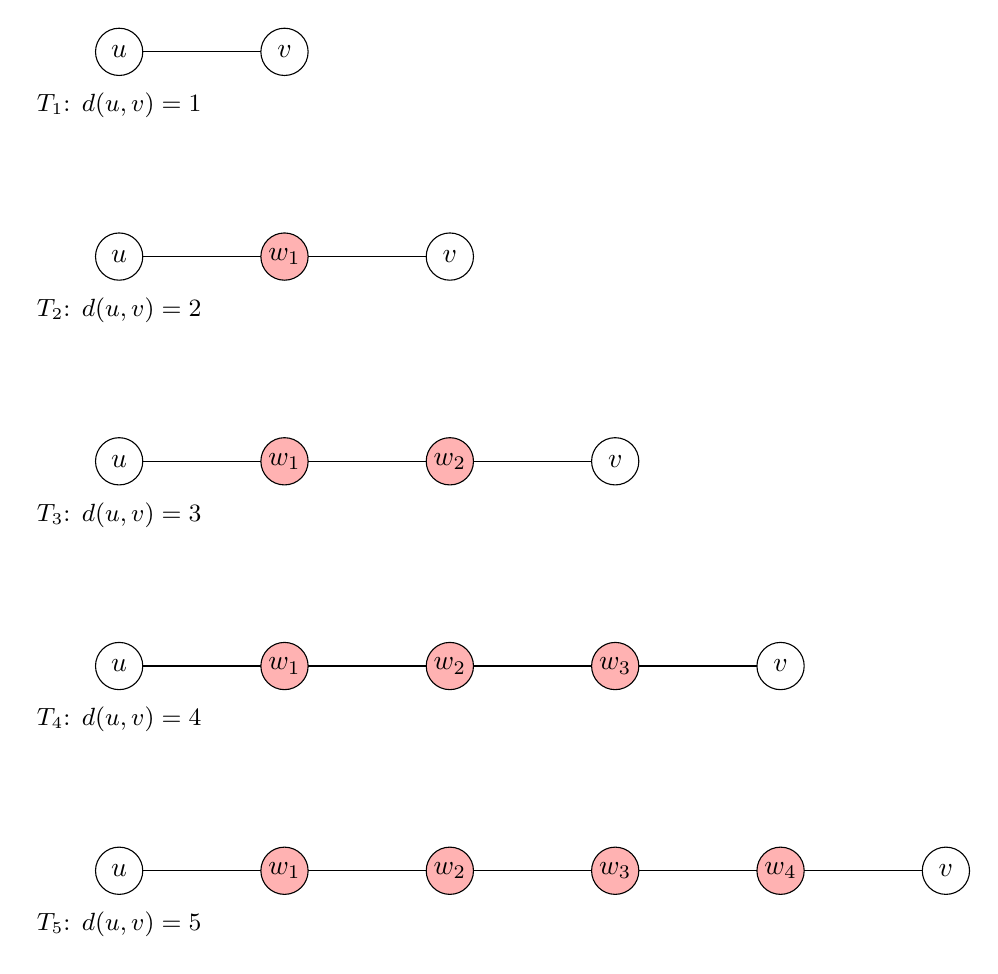
\begin{tikzpicture}[
    node distance=1cm and 1.5cm,
    vertex/.style={circle, draw, minimum size=0.6cm, inner sep=0pt, outer sep=0pt},
    redvertex/.style={vertex, fill=red!30},
    edge/.style={draw, -},
    label/.style={font=\small}
]

% Tree T1 (i=1)
\node[vertex] (T1-u) {$u$};
\node[vertex, right=of T1-u] (T1-v) {$v$};
\draw[edge] (T1-u) -- (T1-v);
\node[label, below=0.1cm of T1-u] {$T_1$: $d(u,v)=1$};

% Tree T2 (i=2)
\node[vertex, below=2cm of T1-u] (T2-u) {$u$};
\node[redvertex, right=of T2-u] (T2-w1) {$w_1$};
\node[vertex, right=of T2-w1] (T2-v) {$v$};
\draw[edge] (T2-u) -- (T2-w1) -- (T2-v);
\node[label, below=0.1cm of T2-u] {$T_2$: $d(u,v)=2$};

% Tree T3 (i=3)
\node[vertex, below=2cm of T2-u] (T3-u) {$u$};
\node[redvertex, right=of T3-u] (T3-w1) {$w_1$};
\node[redvertex, right=of T3-w1] (T3-w2) {$w_2$};
\node[vertex, right=of T3-w2] (T3-v) {$v$};
\draw[edge] (T3-u) -- (T3-w1) -- (T3-w2) -- (T3-v);
\node[label, below=0.1cm of T3-u] {$T_3$: $d(u,v)=3$};

% Tree T4 (i=4)
\node[vertex, below=2cm of T3-u] (T4-u) {$u$};
\node[redvertex, right=of T4-u] (T4-w1) {$w_1$};
\node[redvertex, right=of T4-w1] (T4-w2) {$w_2$};
\node[redvertex, right=of T4-w2] (T4-w3) {$w_3$};
\node[vertex, right=of T4-w3] (T4-v) {$v$};
\draw[edge] (T4-u) -- (T4-w1) -- (T4-w2) -- (T4-w3) -- (T4-v);
\node[label, below=0.1cm of T4-u] {$T_4$: $d(u,v)=4$};

% Tree T5 (i=5)
\node[vertex, below=2cm of T4-u] (T5-u) {$u$};
\node[redvertex, right=of T5-u] (T5-w1) {$w_1$};
\node[redvertex, right=of T5-w1] (T5-w2) {$w_2$};
\node[redvertex, right=of T5-w2] (T5-w3) {$w_3$};
\node[redvertex, right=of T5-w3] (T5-w4) {$w_4$};
\node[vertex, right=of T5-w4] (T5-v) {$v$};
\draw[edge] (T5-u) -- (T5-w1) -- (T5-w2) -- (T5-w3) -- (T5-w4) -- (T5-v);
\node[label, below=0.1cm of T5-u] {$T_5$: $d(u,v)=5$};

\end{tikzpicture}
\caption{Trees \(T_i\) for \(1 \leq i \leq 5\) with vertices \(u\) and \(v\) at distance \(i\), and \(S_i\) (red) as the set of intermediate vertices. Condition \(i\) of Theorem \ref{neccsuff} fails for \(u\) and \(v\) because no vertex in \(S_i\) is adjacent to both.}
\end{figure}

\end{document}